\documentclass[UTF8]{ctexart}
    \title{简单线性回归分析中的概率统计方法综述}
    \author{骆炳君\\
    (软件学院\  2017013573)}
\usepackage{amsmath}
\usepackage{amssymb}
\usepackage{indentfirst}
\usepackage{enumerate}
\usepackage{graphicx} 
% \allowdisplaybreaks[1]
\setcounter{section}{-1}
\begin{document}
\maketitle
\pagenumbering{arabic}

\textbf{摘要:}文章介绍了简单线性回归的模型假设,综述了基于简单线性回归模型进行参数估计、推断和预测的概率统计方法,并在最后总结了基于残差进行模型诊断的思路和方法。

\textbf{关键词:}简单线性回归;回归模型;参数估计;推断;综述

\section{引言}
线性回归分析是利用线性方程对一个或多个自变量和因变量之间关系进行建模的一种回归分析方法,其中自变量个数为一个的模型就是简单线性回归模型。简单线性回归是统计学中最简单的回归模型,也是多元线性回归分析和其他回归分析模型的基础。线性回归分析被广泛运用于趋势分析、流行病学、金融和经济学等领域的研究中,也是机器学习的理论基础之一。

本文在分析简单线性回归模型的过程中,利用了正态分布、t分布、F分布、$\chi^2$分布等概率分布的性质,引入了置信区间、假设检验等统计学概念,应用了最小二乘、极大似然等统计方法,是对本学期概率论与数理统计知识的一次综合运用。

\section{模型}
\subsection{样本数据}
在简单线性回归模型中,样本数据是成对的自变量$X$和因变量$Y$的观测值$(X_i,Y_i)\ i=1,2,\cdots,n$,其中$X_i$是第$i$次观测时的自变量值,$Y_i$是相对应的因变量值,$n$为样本容量。

\subsection{回归方程}
简单线性回归模型认为因变量$Y_i$与自变量$X_i$之间存在如下的线性关系:
\begin{equation}
    Y_i=\beta_0+\beta_1X_i+\epsilon_i
\end{equation}

$\beta_0$是直线的截距,$\beta_1$是直线的斜率,$\beta_0$和$\beta_1$都是模型参数。

$\epsilon_i$是模型中的随机误差项,也是模型中最重要的部分,接下来的分析都将围绕$\epsilon_i$的性质展开。

\subsection{假设}
简单线性回归模型对$\epsilon_i$的概率分布性质做出以下假设:

\begin{enumerate}
    \item $E(\epsilon_i)=0,\ Var(\epsilon_i)=\sigma^2$,$\sigma^2$为模型参数
    \item $\epsilon_i$与$\epsilon_j$$(i\ne j)$之间相互独立
\end{enumerate}

在原模型的基础上,我们提出带正态误差假设的简单线性回归模型,它的假设为

\begin{equation}
    \epsilon_i\ i.i.d.\sim N(0,\sigma^2)
\end{equation}

不难得出,带正态误差假设的模型是原模型的一种特殊情况,它为$\epsilon_i$指定了一个具体的概率分布,这将有助于我们进行后续的推断和预测,由于正态分布在误差分析中的广泛性,这个模型被广泛地应用在实际问题中。在下面的分析中,我们将会体会到这两种模型的不同之处。

\section{参数估计}
模型中的参数有$\beta_0$、$\beta_1$和$\sigma^2$,记$b_0=\hat{\beta_0}$,$b_1=\hat{\beta_1}$,在下面的推导中可以得到,$b_0$与$b_1$满足关系
$$\bar{Y}=b_0+b_1\bar{X}$$

在参数估计中我们将重点研究$\beta_1$和$\sigma^2$的估计。

\subsection{$\beta_1$的估计}
\subsubsection{最小二乘估计}
最小二乘估计对$\epsilon_i$的分布没有要求,因而适用于一般的简单线性回归模型。记第$i$次观测时的残差为
$$e_i=Y_i-\hat{Y}_i=Y_i-\beta_0-\beta_1X_i$$

在最小二乘估计中,用残差平方和$Q$来评估模型的拟合度。
$$Q=\sum_{i=1}^ne_i^2=\sum_{i=1}^n(Y_i-\beta_0-\beta_1X_i)^2$$

因此优化目标就是得到使$Q$最小时的$\beta_0$和$\beta_1$的值,将$Q$对$\beta_0$、$\beta_1$求导,可以得到

\begin{equation}
\left\{
\begin{aligned}
&\frac{\partial Q}{\partial \beta_0} = -2\sum_{i=1}^ne_i=0 \\
&\frac{\partial Q}{\partial \beta_1} = -2\sum_{i=1}^nX_ie_i=0
\end{aligned}
\right.
\end{equation}

求解这个方程可得
\begin{equation}
b_1=\frac{\sum_{i=1}^n(X_i-\bar{X})(Y_i-\bar{Y})}{\sum_{i=1}^n(X_i-\bar{X})^2},\ b_0=\bar{Y}-b_1\bar{X}
\end{equation}

\subsubsection{最大似然估计}
最大似然估计依赖于密度函数,因此仅适用于带正态误差假设的简单线性回归模型。在模型中,由(2)中的假设可得似然函数
$$L=\frac{1}{(2\pi\sigma^2)^{n/2}}\exp\{-\frac{\sum_{i=1}^ne_i^2}{2\sigma^2}\}$$

由最大似然方法可得
$$b_0,b_1,\hat{\sigma}^2=\arg\max L=\arg\min(-\log L)$$

最终得到$\beta_0$、$\beta_1$的最大似然估计与(4)相同,同时可得到$\sigma^2$的最大似然估计
$$\hat{\sigma}^{2,ml}=\frac{\sum_{i=1}^2e_i^2}{n}$$

\subsubsection{性质}
由(4)可得
\begin{equation}
    E(b_1)=\frac{\sum\beta_1(X_i-\bar{X})^2}{\sum(X_i-\bar{X})^2}=\beta_1
\end{equation}

所以$b_1$是$\beta_1$的无偏估计,同理可证明$b_0$也是$\beta_0$的无偏估计,另外还可以证明,$b_0$和$b_1$是$\beta_0$和$\beta_1$的最佳线性无偏估计。

\subsection{$\sigma^2$的估计}
残差$e_i$是误差的观测值,所以可以考虑用残差平方和SSE(Sum of Squared Errors)来估计$\sigma^2$,但由于模型假设所导出的(3)式的限制,使得n个$e_i$之间并不是相互独立的,其真实的自由度$df_E=n-2$,因此
\begin{equation}
    \hat{\sigma}^2=\frac{SSE}{df_E}=\frac{\sum_{i=1}^ne_i^2}{n-2}
\end{equation}

$SSE/df_E$又被称为MSE(Mean of Squared Errors)。可以证明,MSE是$\sigma^2$的无偏估计。

\section{参数推断}
本部分主要研究$\beta_1$的参数推断,而这依赖于估计值$b_1$的具体分布,所以下面的分析都将在正态误差的假设下进行。

\subsection{$b_1$的分布}
由(4)式,$b_1$是相互独立的正态分布的线性组合,由正态分布的性质可知,$b_1$也一定服从正态分布。

由(5)式已经得到了$E(b_1)$,又有

\begin{align*}
b_1&=\frac{\sum_{i=1}^n(X_i-\bar{X})Y_i}{\sum_{i=1}^n(X_i-\bar{X})^2}\\
&=\frac{\sum_{i=1}^n(X_i-\bar{X})(\beta_0+\beta_1X_i+\epsilon_i)}{\sum_{i=1}^n(X_i-\bar{X})^2}\\
&=\beta_1+\frac{\sum_{i=1}^n(X_i-\bar{X})\epsilon_i}{\sum_{i=1}^n(X_i-\bar{X})^2}
\end{align*}

$$Var(b_1)=\frac{\sum_{i=1}^n(X_i-\bar{X})^2Var(\epsilon_i)}{(\sum_{i=1}^n(X_i-\bar{X})^2)}=\frac{\sigma^2}{\sum_{i=1}^n(X_i-\bar{X})^2}$$


所以
\begin{equation}
    b_1\sim N(\beta_1,\frac{\sigma^2}{\sum_{i=1}^n(X_i-\bar{X})^2})
\end{equation}

\subsection{$\beta_1$的显著性检验}
在面向实际问题进行建模时,首先需要确定某个自变量是否有必要被加入模型中,即它对因变量是否有足够显著的解释能力,因而引入显著性检验问题:
$$H_0:\beta_1=0\leftrightarrow H_a:\beta_1\ne0$$

取检验统计量
$$T=\frac{b_1}{s^2/\sum_{i=1}^n(X_i-\bar{X})^2}$$

则在$H_0$下,$T\sim t_{n-2}$

因此在给定显著性水平$\alpha$的条件下,可构造拒绝域
$$\{T: |T|>t_{n-2}(1-\alpha/2)\}$$

当$|T|>t_{n-2}(1-\alpha/2)$时,拒绝原假设$H_0$,认为$\beta_0$在模型中是显著的。


\subsection{$\beta_1$的一般假设检验和置信区间}
对显著性检验问题进行拓展,就可以得到一般的假设检验问题:
$$H_0:\beta_1=\mu\leftrightarrow H_a:\beta_1\ne\mu$$

可构造检验统计量
$$T_0=\frac{b_1-\mu}{s^2/\sum_{i=1}^n(X_i-\bar{X})^2}$$

此后的检验过程与判定准则均与3.2中相同。

假设检验问题和置信区间问题在本质上是等价的,因此可同理构造枢轴变量
$$T_1=\frac{b_1-\beta_1}{s^2/\sum_{i=1}^n(X_i-\bar{X})^2}\sim t_{n-2}$$

在置信水平为$\beta$的情况下,可构造$\beta_1$的置信区间
$$[b_0-t_{n-2}(1-\beta/2)s^2/\sum_{i=1}^n(X_i-\bar{X})^2,b_0+t_{n-2}(1-\beta/2)s^2/\sum_{i=1}^n(X_i-\bar{X})^2]$$

\section{预测分析}
建立简单线性回归模型的目的通常是做出预测,预测值的方差则决定了这个预测值的可靠程度,也是进行区间估计和假设检验的基础,本部分内容将对给定自变量的某个值$X_h$时所对应的因变量的期望$E(Y_h)$和实际观测值$Y_{h(new)}$的预测值,着重对预测值的方差进行分析。

\subsection{$E(Y_h)$的分析}
记$\mu_h=E(Y_h)$,在$X=X_h$处,
$$\mu_h=\beta_0+\beta_1X_h$$

将模型参数用它们的估计值替代,就得到了$\mu_h$的估计
$$\hat{\mu}_h=b_0+b_1X_h=\bar{Y}+(b_1X_h-\bar{X})$$

可得
$$E(\hat{\mu}_h)=\mu_h$$

$$Var(\hat{\mu}_h)=\sigma^2(\frac{1}{n}+\frac{(X_h-\bar{X})^2}{\sum_{i=1}^n(X_i-\bar{X})^2})$$

因为$\hat{\mu}_h$是相互独立的正态分布的线性组合,所以可得$\hat{\mu}_h$服从正态分布且
$$\hat{\mu}_h\sim N(\beta_0+\beta_1X_h,\sigma^2(\frac{1}{n}+\frac{(X_h-\bar{X})^2}{\sum_{i=1}^n(X_i-\bar{X})^2}))$$

\subsection{$Y_{h(new)}$的分析}
由模型假设(1)式可得,
$$Y_h=\mu_h+\epsilon=\beta_0+\beta_1X_h+\epsilon,\ \epsilon\sim N(0, \sigma^2)$$

代入$\mu_h$的估计值,可得$Y_{h(new)}$的估计
$$\hat{Y}_{h(new)}=\hat{\mu}_h+\epsilon=b_0+b_1X_h+\epsilon$$

相比$\hat{\mu}_h$,$\hat{Y}_{h(new)}$的期望不变,但是方差却多出了新增的$\epsilon$的部分,因此
$$Var(\hat{Y}_{h(new)})=\sigma^2(1+\frac{1}{n}+\frac{(X_h-\bar{X})^2}{\sum_{i=1}^n(X_i-\bar{X})^2})$$

同理可得,$\hat{Y}_{h(new)}$服从正态分布且
$$\hat{Y}_{h(new)}\sim N(\beta_0+\beta_1X_h, \sigma^2(1+\frac{1}{n}+\frac{(X_h-\bar{X})^2}{\sum_{i=1}^n(X_i-\bar{X})^2})$$

\section{评估与诊断}
对线性回归模型进行建模的基础是(2)式中的假设,因此在实际问题中需要评估数据是否满足满足这些假设,并对模型存在的问题进行诊断。由于模型假设主要集中于误差项$\epsilon$,在评估与诊断中也将主要对残差$e$的分布性质进行分析。这一部分的内容涉及的概率统计理论较少,但在应用情景中非常重要。

\subsection{正态性问题}
模型中假设了$\epsilon$服从正态分布,这是进行一系列推断和检验的基础,如果不满足这个假设,那么置信区间、假设检验和预测分析的可靠度都将受到影响。

在数据处理中,可使用Normal Q-Q图(Normal Quantile Plots)来评估$\epsilon$的正态性,其原理是将正态分布的理论分布和样本$e$的实际分布作为两个坐标轴作图,若$\epsilon$服从正态分布,那么图上的点应该近似为直线。

\begin{figure}[htbp]
	\centering
	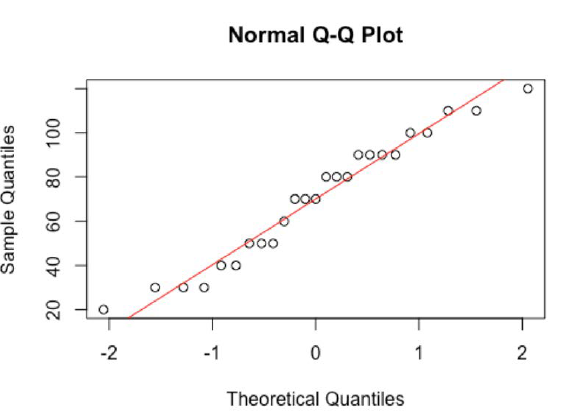
\includegraphics[width=0.7\linewidth]{plot1.png}
\end{figure} 

\subsection{异方差问题}
误差的异方差性也是模型评估的关注点,这类问题通常是由于误差$\epsilon$的方差与自变量$X$有关而导致的。这类问题可以通过$e\sim X$图,观察残差与自变量间是否存在显著关联来进行评估。例如下图中的模型,就出现了比较严重的异方差问题。

\begin{figure}[htbp]
	\centering
	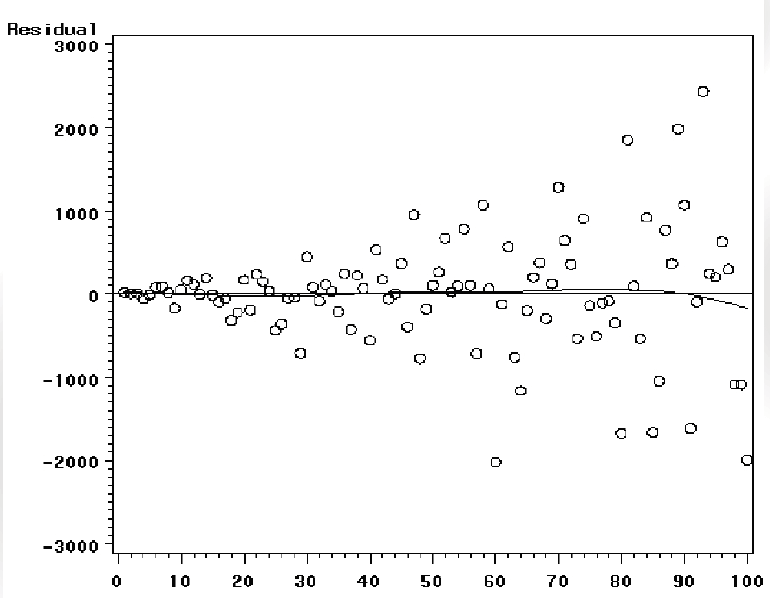
\includegraphics[width=0.7\linewidth]{plot2.png}
\end{figure} 

\begin{thebibliography}{99}
    \bibitem{ref1}Senter H F . Applied Linear Statistical Models (5th ed.). Michael H. Kutner, Christopher J. Nachtsheim, John Neter, and William Li[J]. Journal of the American Statistical Association, 2008, 103(June):880-880.  
    \bibitem{ref2}Hocking R R . Methods and Applications of Linear Models: Regression and the Analysis of Variance, 2nd Edition[J]. Computational Statistics \& Data Analysis, 2013, 26(3):378-379.
\end{thebibliography}

\end{document}